\section{Evaluation}
\label{Section: experiment}

\subsection{Dataset and Metric}
\label{subsec: datasets}

Most public sources datasets cannot fully satisfy all configuration choices, for example, some can only guarantee 30 frames but cannot guarantee 1024p resolution. In contrast, others can ensure resolution but cannot provide a sufficient frame rate. Still, in recent years, most of the driving recorder can provide enough resolution and frame rate, so we try to use Youtube video as fellows. We selected three datasets: M6, Duke, and Multi-Camera Dataset. M6 was taken from a traffic camera on the longest motorway in Britain. Duke is a video from a fixed camera placed at an intersection, and  the traffic flow in the video increases or decreases periodically as the traffic light change. Since the first two datasets were sourced from a fixed camera, to ensure that AutoConfigure still performs better when road conditions change dramatically, we used three videos collected from the dashcam. We combined them into one video, Multi-Camera Dataset.

For metric, we use the F1 score as the accuracy and average GPU processing time per frame as the resource consumption, detail described in Section \ref{subsec: formulation}.
%First, in order to eliminate the bias caused by Cookies and personal preferences, we use private browsing mode to search keywords (e.g., "drivecam highway hd"). Second, manually delete irrelevant videos (e.g., ads for some driving recorders) and download videos that are longer than ten minutes. In addition, these videos need to be as dynamic as the real world, such as not standing still for too long. Becaues of none of these videos contained ground truth, we used the data of the original video output from DNN as the tags to calculate the accuracy. For instance, in object detection, the accuracy is defined by the F1 score with respect to the server-side DNN output in highest resolution (original) with over 50$\%$ confidence score.Based on the above filtering strategy, we finally selected three datasets: 

%we selected three datasets:
%M6: The M6 is the longest motorway in Britain and the most important road from the Midlands to the West Coast. Thousands of cars travel on it every day. This video was taken from a traffic camera, and its natural dynamics allows us to experiment with this video.
%
%Duke: Duke is a video from a fixed camera placed at an intersection. Because it is fixed in the middle of the intersection, the traffic flow in the video increases or decreases periodically as the traffic light change.
%
%Mutli Camera Dataset: Since the first two datasets were sourced from a fixed camera, in order to ensure that AutoConfigure still has better performance when road conditions change dramatically, we used three videos collected from the dashcam, and since they are relatively similar, we combined them into one video.

\begin{figure*}[!t]
	\begin{minipage}[t]{0.32\linewidth}
		\centerline{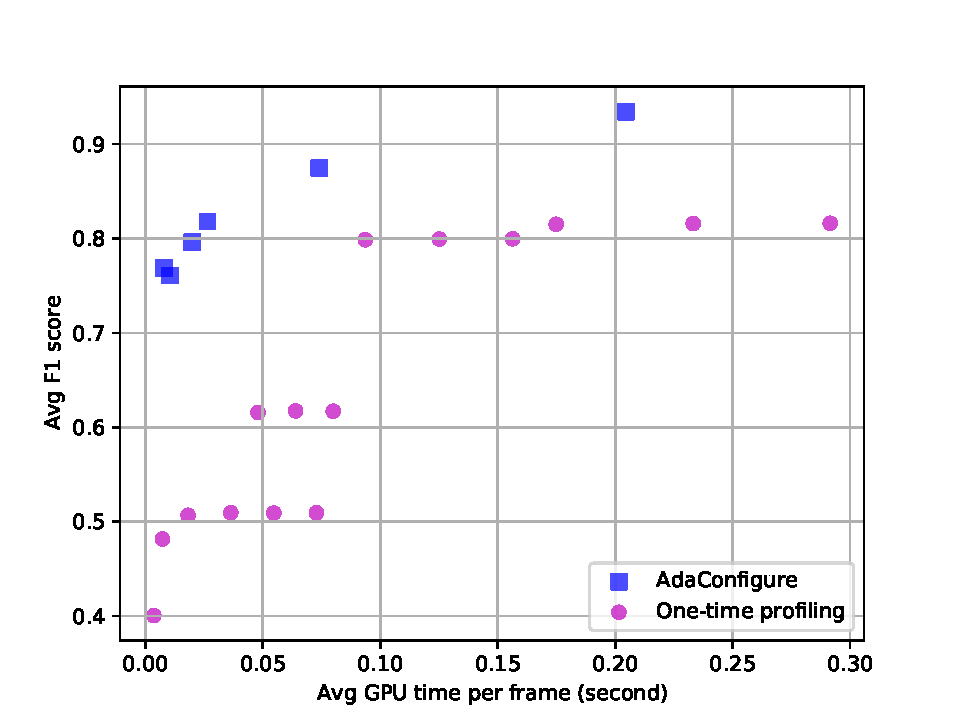
\includegraphics[width=6.5cm]{figures/m6.pdf}}
		\centerline{(a) M6}
	\end{minipage}
	\hfill
	\begin{minipage}[t]{0.32\linewidth}
		\centerline{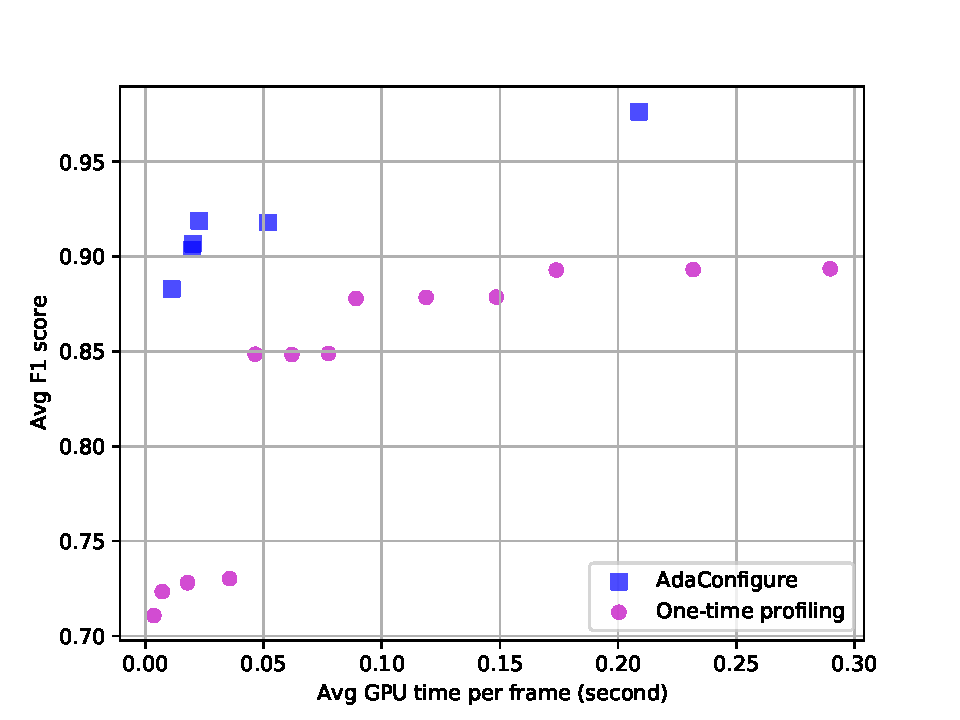
\includegraphics[width=6.5cm]{figures/duke.pdf}}
		\centerline{(b) Duke}
	\end{minipage}
	\hfill
	\begin{minipage}[t]{0.32\linewidth}
		\centerline{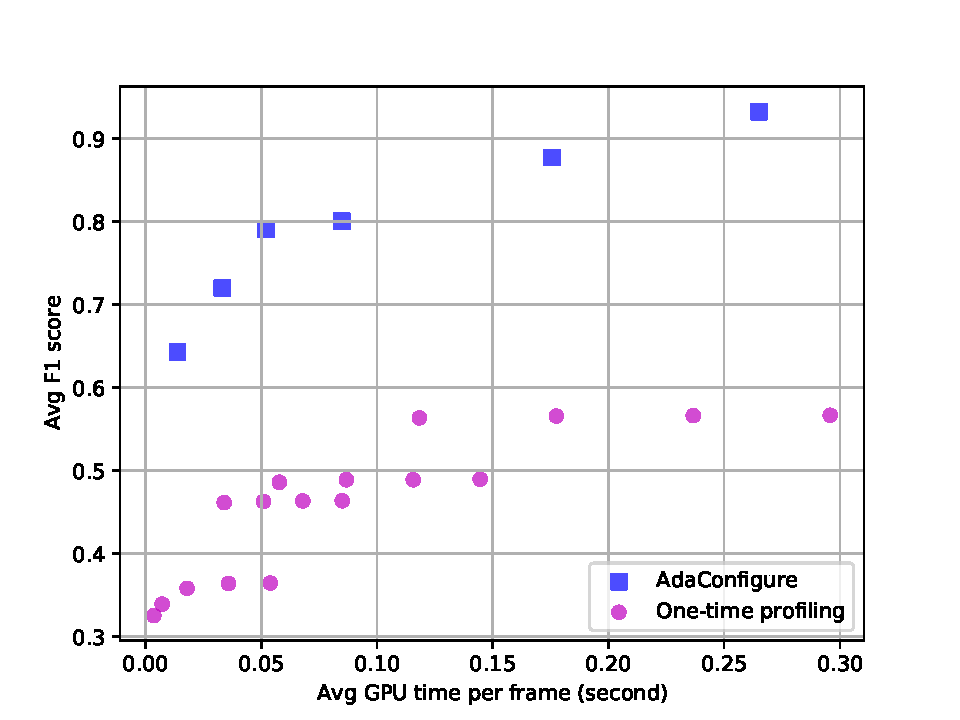
\includegraphics[width=6.5cm]{figures/_Westbound_Eastbound_Rear.pdf}}
		\centerline{(c) Multi-Camera Dataset}
	\end{minipage}		
	\caption{AutoConfigure (blue) consistently outperforms the baseline of one-time profiling (magenta) across different datasets. Each dot represents the results of running each solution.}
	\label{fig: results}
\end{figure*}

\subsection{Configuration Selection}
\label{subsec: configuration}
We simulate the environment \cite{trade-offs} with three pretrained object detection models in Tensorflow, which are SSD+ResNet152V1, FasterRCNN+ResNet50V1, FasterRCNN+InceptionResNetV2. For each model, two kinds of image resolution, which is $1024\times1024$ and $640\times640$, can be picked up. In our experiment, we set the choices space of fps as \{1, 2, 5, 10, 15, 20, 25, 30\}. We FFmpeg \cite{ffmpeg} to switch the frame rate and image resolution, which decide which frames and in what size they should be fed to the object detection model. The configuration space comprises all possible combinations of values of these knobs, so the environment has 48 configurations in total.

\subsection{Experiment Parameters}
We apply a deep Q-learning network policy to train the agent. In the training procedure, we build up to eight independently identical environments for each data set to speed up the training and decrease the data's dependency. The leaning rate is set to 0.001. For each dataset, we train the agent 10 epochs and 1000 steps per epoch. Some important hyperparameters in our experiments are given in Table ~\ref{tab: parameters}.

\begin{table}[!t]
	\centering
	\label{tab: parameters}
	%     \begin{tabular}{llllll}
	\resizebox{0.4\textwidth}{!}{
		\begin{tabular}{cccccc}
			\toprule
			Notation          & Value & & & Notation     & Value  \\ \midrule
			$\epsilon$    & 0.8    & & & $k_1$      & 3   \\
			$\gamma$      & 0.9  & & & $k_2$    & 3    \\
			$ \beta $ & 0.2,0.3,...,0.9 & & & $ T (train) $ & 1  \\
			$ t(inference)  $  &  1   & & &   $ T (inference)  $  &  4      \\ 
	\end{tabular}}
	\caption{Experiment parameter}
	\label{tab: parameters}
	%	\vspace{-0.5cm}
\end{table}

\subsection{Experiment Results}
We evaluate AutoConfigure on M6, Duke, and Multi-Camera Dataset video streams. Figure \ref{fig: results} shows that AutoConfigure consistently outperforms the baseline of static configuration (profiling configurations once at the beginning of a video stream) along with resource consumption and several accuracy metrics on different datasets. Each magenta dot represents one static configuration solution. These static configuration solutions including some expensive configurations, such as \{FasterRCNN+InceptionResNetV2, 640p, 30fps\}, \{FasterRCNN+ResNet50V1, 1024p, 25fps\}, and some cheap configurations, such as \{SSD+ResNet152V1, 640p, 1fps\}, \{SSD+ResNet152V1, 640p, 2fps\}, \{SSD+ResNet152V1, 640p, 5fps\}. Each blue dot represents one AutoConfigure configuration solution, which is dependent on the balance factor $\beta$ in reward function, presented in Section \ref{subsec: reward}. The detailed discussion about differents AutoConfigure solutions is in Section . As shown in Figure \ref{fig: results}(a)(b), AutoConfigure achieves 10-30\% higher accuracy with a similar amount of resources, or achieve a similar accuracy with only 50-80\% of the resources on a single-camera dataset. As shown in Figure \ref{fig: results}(c), the gap between AutoConfigure and static configuration is larger than Figure \ref{fig: results}(a)(b), indicating that AutoConfigure has a better improvement on the multi-camera situation. AutoConfigure achieves 25-35\% higher accuracy with a similar amount of resources, or achieve higher accuracy with only 75-85\% of the resources on Multi-Camera Dataset. In a word, AutoConfigure can improve 10-35\% higher accuracy or save 50-85\% resource consumption.

\subsubsection{Different AutoConfigure Solutions}
\label{subsec: different sulutions}
In the training phase, when using different balance factors $\beta$ in the reward function, we would obtain different agents (different automatic configuration strategies). In general, the $\beta$ is bigger, indicating the accuracy is more important relatively, and the agent would choose a more expensive configuration. In our experiment, we set $\beta$ is 0.2,0.3,...,0.9, and the results of different AutoConfigure solutions on Multi-Camera Dataset are listed in Table \ref{tab: different sulutions}.

\begin{table}[!t]
	\centering
	%     \begin{tabular}{lll}
	\resizebox{0.4\textwidth}{!}{
		\begin{tabular}{ccc}
			\toprule
			balance factor $\beta$ & Avg GPU time per frame (second) & Avg F1 score  \\ \midrule
			0.2          & 0.01384  &  0.64307            \\
			0.3          & 0.03314  &  0.72008            \\
			0.4          & 0.04921  &  0.78920            \\
			0.5          & 0.05203  &  0.79096            \\
			0.6          & 0.08479  &  0.80056            \\
			0.7          & 0.17570  &  0.87731            \\
			0.8          & 0.26511  &  0.93262            \\
			0.9          & 0.30937  &  0.96537           \\
			\bottomrule
	\end{tabular}}
	\caption{Resource consumption and F1 accuracy for different AutoConfigure solutions}
	\label{tab: different sulutions}
	% \vspace{-0.5cm}
\end{table}

Table \ref{tab: different sulutions} shows that when the $\beta$ increases, the resource consumption and the accuracy of the corresponding solution both would increase, indicating the AutoConfigure solutions of big $\beta$ would choose the more expensive configuration to inference. We can leverage this to train proper configuration strategy for different service demands, for example, using big $\beta$ for high-accuracy demand services and using small $\beta$ for low-accuracy demand services.  

\subsubsection{Profile Cost}
\label{subsec: profile cost}
Comparing to the static solution that profiles configurations once, in our solution, the video
chunk is passed to the AutoConfigure firstly to estimate the configuration. Running this RL agent brings profile cost (extra resource consumption) to the whole system. In this section, we evaluate this profile cost. In the inference phase, we divide the video into $T$-second intervals as video chunks and use AutoConfigure to choose the proper configuration for the first t seconds of the video chunk. It then sticks with the chosen configuration for the rest of the video chunk, i.e., for $T-t$ seconds. We use T = 4 and t = 1 for our experiments. The profile cost, including the resource of extract $k_1$ embeddings and the cost of agent choosing actions. In our test, the average time of extract one embedding is 0.02s, and the average time of agent choosing action is 0.0006s, which can be ignored. We compute the ratio by dividing profile time into total inference time, which is equals the frame number multiply the average time per frame. The profile time is about 0.1-1\% of the overall video analytics resource consumption. The concrete ratio depends on the concrete AutoConfigure configuration solutions, such as the solutions listed in Table \ref{tab: different sulutions}.        

%\begin{table}[!t]
%%\begin{table}[H]
%	\centering
%	%     \begin{tabular}{lll}
%	\resizebox{0.5\textwidth}{!}{
%		\begin{tabular}{lcc}
%			\toprule
%			Model and Image size & Inference time & Accuracy  \\ \midrule
%			SSD MobileNetV2 320p          & 49.5 ms  &  xxx            \\
%			SSD MobileNetV2 640p          & 58.5 ms  &  0.494            \\
%			SSD ResNet152V1 640p          & 100 ms  &  0.579            \\
%			SSD ResNet152V1 1024p          & 182.3 ms  &  0.614            \\
%			FasterRCNN ResNet50V1 640p          & 106.4 ms  &  0.637            \\
%			FasterRCNN ResNet50V1 1024p          & 120.5 ms  &  0.786           \\
%			FasterRCNN InceptionResNetV2 640p          & 361.8 ms  &  0.734            \\
%			FasterRCNN InceptionResNetV2 1024p          & 418.4 ms  &  1            \\
%			\bottomrule
%	\end{tabular}}
%	\caption{Inference time and F1 for different models and resolutions car truck}
%	\label{tab: latency-overhead}
%	% \vspace{-0.5cm}
%\end{table}
%
%\begin{table}[!t]
%	%\begin{table}[H]
%	\centering
%	%     \begin{tabular}{lll}
%	\resizebox{0.5\textwidth}{!}{
%		\begin{tabular}{lcc}
%			\toprule
%			Model and Image size & Inference time & Accuracy  \\ \midrule
%			SSD MobileNetV2 320p          & 49.5 ms  &  xxx            \\
%			SSD MobileNetV2 640p          & 58.5 ms  &  0.753            \\
%			SSD ResNet152V1 640p          & 100 ms  &  0.886            \\
%			SSD ResNet152V1 1024p          & 182.3 ms  &  0.942            \\
%			FasterRCNN ResNet50V1 640p          & 106.4 ms  &  0.889            \\
%			FasterRCNN ResNet50V1 1024p          & 120.5 ms  &  0.98           \\
%			FasterRCNN InceptionResNetV2 640p          & 361.8 ms  &  0.965            \\
%			FasterRCNN InceptionResNetV2 1024p          & 418.4 ms  &  1            \\
%			\bottomrule
%	\end{tabular}}
%	\caption{Inference time and F1 for different models and resolutions}
%	\label{tab: latency-overhead}
%	% \vspace{-0.5cm}
%\end{table}

%\begin{figure}[!t]
%	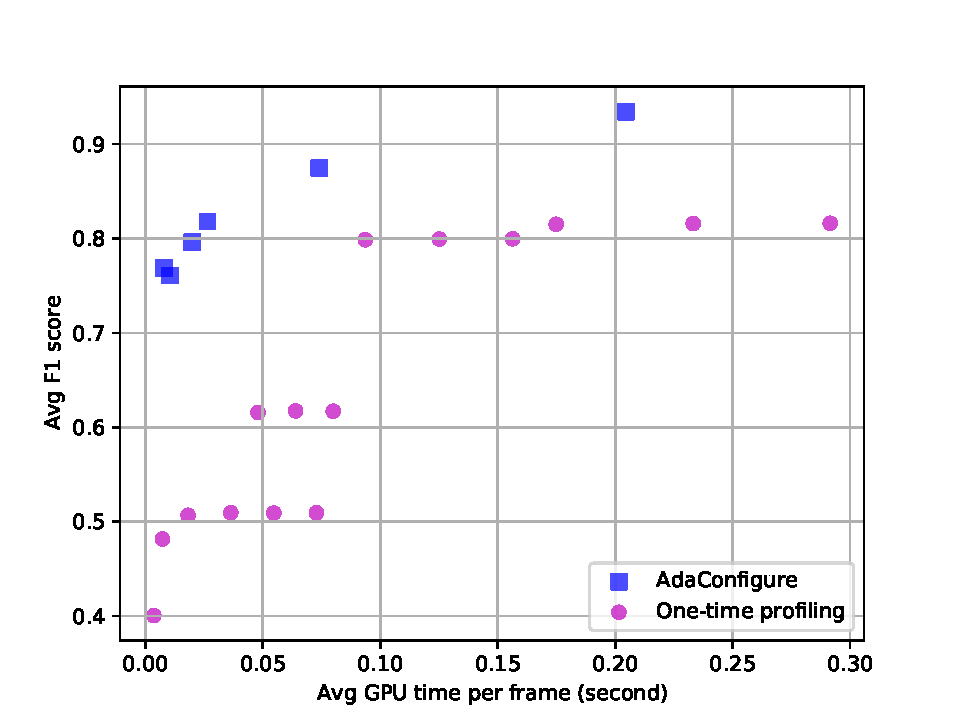
\includegraphics[width=9cm,height=8cm]{figures/m6.pdf}
%	\centering
%	\caption{The effect of different models, frame rate, and resolutions on accuracy and processing time. AutoConfigure (blue) consistently outperforms the baseline of one-time update (magenta) across different datasets. Each dot represents the results of running each solution.}
%	\label{fig_m6}
%\end{figure}